% SwarmX manuscript prepared for submission to SoftwareX.
% Bibliography: Better BibTeX export plus manuscript-local vetted additions.
\documentclass[preprint,12pt,a4paper]{elsarticle}

\usepackage[T1]{fontenc}
\usepackage{booktabs}
\usepackage{tabularx}
\usepackage{array}
\usepackage{graphicx}
\usepackage{xcolor}
\usepackage{tikz}
\usetikzlibrary{arrows.meta,positioning}
\usepackage{float}
\usepackage[section]{placeins}
\usepackage{xurl}
\usepackage[hidelinks]{hyperref}
\pdfstringdefDisableCommands{\def\corref#1{}}
\hypersetup{pdfauthor={Ziya Tang and Xiangchao Gan}}
\usepackage{microtype}
\setlength{\parindent}{0pt}

\journal{SoftwareX}
\biboptions{sort&compress}

\newcolumntype{Y}{>{\raggedright\arraybackslash}X}
\newcolumntype{C}{>{\centering\arraybackslash}X}

\begin{document}

\begin{frontmatter}

% 中文：SwarmX：面向科研智能体工作流的可追溯编排
\title{SwarmX: Traceable Orchestration for Scientific Agent Workflows}

% 中文：作者、单位与通讯作者。
\author[1]{Ziya Tang}
\ead{tang@stu.njau.edu.cn}
\author[1]{Xiangchao Gan\corref{cor1}}
\ead{gan@njau.edu.cn}
\cortext[cor1]{Corresponding author}
\affiliation[1]{
  organization={Nanjing Agricultural University},
  city={Nanjing},
  country={China}
}

\begin{abstract}
Agent-assisted research produces records across conversations, computations and files, but their
fragmentation makes findings difficult to trace and reuse across sessions. SwarmX is open-source
software that links these records while preserving native agent sessions. It links revisioned
research records and content-addressed artifacts to source-linked memory, with recursive delegation
across agents and configurable approval for memory writes. A guided synthetic-data example
demonstrates software integration through figure generation, recomputation in a separate session,
claim recording, memory write approval and retrieval in a later session. Integration tests and artifact
checks validate the recorded workflow and persistence boundaries. SwarmX supports inspection of
the evidence underlying research findings and reuse of source-linked knowledge across sessions.
\end{abstract}

% 中文：关键词：科研软件；大语言模型智能体；科研工作流；多智能体编排；科研溯源；RO-Crate
\begin{keyword}
research software \sep LLM agents \sep scientific workflows \sep multi-agent orchestration
\sep research provenance \sep RO-Crate
\end{keyword}

\end{frontmatter}

% 中文：代码元数据
\section*{Required Metadata}
\section*{Current code version}

% 中文：软件描述、实例和截图对应固定实现版本。
Table~\ref{tab:code-metadata} identifies the frozen implementation used for the current
workflow and screenshots in Section~\ref{sec:examples}.

\begin{table}[H]
\centering
\caption{Code metadata for SwarmX 0.1.0, source revision \texttt{9e1e818}.}
\label{tab:code-metadata}
\footnotesize
\renewcommand{\arraystretch}{1.08}
\begin{tabularx}{\textwidth}{@{}p{0.055\textwidth}p{0.31\textwidth}Y@{}}
\toprule
\textbf{ID} & \textbf{Code metadata description} & \textbf{Metadata} \\
\midrule
C1 & Current code version & \texttt{0.1.0} \\
C2 & Permanent GitHub link to code/repository used for this code version &
\href{https://github.com/tcztzy/swarmx/tree/9e1e818acd438dcbf30fb9dc46d758495d24d094}{Source revision \texttt{9e1e818}} \\
C3 & Legal Code License & MIT License \\
C4 & Code versioning system used & Git \\
C5 & Software code languages, tools, and services used & TypeScript, Node.js, Electron, SQLite, Rust/Typst, upstream ACP adapters, Docker/Jupyter Data Science, Zotero, Git, and DVC \\
C6 & Compilation requirements, operating environments \& dependencies & Node.js and pnpm as declared in the pinned manifests; stable Rust and a C/C++ linker for the bundled Typst runtime; Docker for Python execution. macOS requires Xcode command-line tools. Native conversation requires provider credentials; literature and versioned-data features require Zotero and Git/DVC. Linux and macOS are CI targets. \\
C7 & If available Link to developer documentation/manual & \href{https://github.com/tcztzy/swarmx}{Repository README} and versioned developer documentation \\
C8 & Support email for questions & \href{mailto:gan@njau.edu.cn}{gan@njau.edu.cn} \\
\bottomrule
\end{tabularx}
\end{table}

% 中文：动机与重要性
\section{Motivation and significance}
\label{sec:motivation}

Agent-assisted research combines activities such as literature search, computation, hypothesis
development and manuscript preparation~\cite{lu2026,gottweis2026,swanson2025}. A result may depend
on conversation history, notebook executions, workspace files, review decisions and knowledge
carried into later sessions. These records have different storage locations and lifecycles.
A transcript alone does not identify which artifact version supports a claim; a file tree does
not explain why that output was accepted; and a workflow log does not preserve its later use.
This fragmentation makes it difficult to inspect a finding, resume a project or hand work
to another researcher.

Computational-provenance systems preserve important parts of this record. Whole Tale captures
reproducible environments, AiiDA manages workflows, noWorkflow captures Python execution and
ProvBook enriches notebooks~\cite{brinckman2019,pizzi2016,pimentel2017,samuel2018}.
Workflow Run RO-Crate packages executions, while PROV-AGENT represents agent
interactions~\cite{leo2024,souza2025a}. Claim-oriented systems address the interpretation of
such records: ResearchLoop controls claim admission through evidence gates, and LEDGER,
artifact-centered observability and PaperTrail support audit graphs, lineage and
review~\cite{xia2026,kim2026,yin2026,martin-boyle2026}. Together, these approaches motivate
explicit links between the process that produced an output and the claim it supports.

Carrying a finding into a later session adds a further requirement: the reusable knowledge must
retain those links as its sources change. Retrieval-augmented generation and Self-RAG supply
external knowledge during generation~\cite{lewis2020rag,asai2023selfrag}; Reflexion, Voyager
and Agent Workflow Memory retain feedback, skills and procedures for subsequent
tasks~\cite{shinn2023reflexion,wang2023voyager,wang2024workflowmemory}. For a continuing research
project, retrieval therefore needs to be connected to the source versions, review decisions
and corrections associated with a saved finding. Table~\ref{tab:related} situates this
record-management task among the adjacent systems.

SwarmX connects native agent sessions, scientific records and reusable memory. Its contribution
is an inspectable path from a saved finding to the cited source revisions and the recorded
computations associated with its evidence. Individual agents and delegated teams use the same
records and curation operations. The FAIR principles and RO-Crate guide portable representation
and exchange~\cite{wilkinson2016,soiland-reyes2022}; native runtimes, scientific services and
the knowledge store retain responsibility for their respective records.

This article presents the architecture for linking these records, the controls for creating
and revising sourced knowledge, and a reproducible demonstration of the resulting workflow.
Integration tests and artifact checks establish the implemented behavior and its persistence
boundaries.

\begin{table}[!htbp]
\centering
\caption{Records emphasized by adjacent systems and the scope of SwarmX.}
\label{tab:related}
\scriptsize
\renewcommand{\arraystretch}{1.12}
\begin{tabularx}{\textwidth}{@{}>{\raggedright\arraybackslash}p{0.25\textwidth}>{\raggedright\arraybackslash}p{0.20\textwidth}YY@{}}
\toprule
\textbf{Work} & \textbf{Primary records} & \textbf{Supported activity} & \textbf{SwarmX scope} \\
\midrule
Whole Tale; AiiDA; noWorkflow; ProvBook~\cite{brinckman2019,pizzi2016,pimentel2017,samuel2018} & Environments, workflows, scripts, notebooks & Execution provenance and reproducible computation & Links outputs to claims and native sessions \\
Workflow Run RO-Crate; PROV-AGENT~\cite{leo2024,souza2025a} & Execution and interaction graphs & Provenance representation and exchange & Connects research revisions, exports and curated memory \\
ResearchLoop; LEDGER; artifact-centered observability; PaperTrail~\cite{xia2026,kim2026,yin2026,martin-boyle2026} & Claims, evidence and audit records & Claim admission, lineage and inspection & Retains links from running workflows through later knowledge retrieval \\
RAG; Self-RAG~\cite{lewis2020rag,asai2023selfrag} & Retrieved passages & Generation supported by external knowledge & Supplies knowledge with scope, revision and write controls \\
Reflexion; Voyager; Agent Workflow Memory~\cite{shinn2023reflexion,wang2023voyager,wang2024workflowmemory} & Feedback, skills and procedures & Experience accumulation and reuse & Links saved knowledge to scientific source revisions \\
\bottomrule
\end{tabularx}
\end{table}
\FloatBarrier

% 中文：软件描述
\section{Software description}
\label{sec:software}

% 中文：先解释执行、证据与记忆的联系，再说明记录的归属。
\subsection{Software architecture}
\label{sec:architecture}

SwarmX connects records through explicit identifiers and source references
(Figure~\ref{fig:architecture}). Tool results link an observed agent execution to scientific
entity revisions and registered artifacts. Evidence relations connect those objects to a claim;
a memory concept can cite the corresponding source revision when carrying the finding into
another session. These links let a reader work back from retrieved knowledge to its recorded
evidence.

The data model draws on Mokyr's distinction between propositional and prescriptive
knowledge~\cite{mokyr2005}. Questions, hypotheses, claims and evidence describe the basis of
a finding; code, notebook cells and experiment runs describe its production. Revisioned
locators and content digests connect the two families of records.

Record ownership follows these responsibilities. Native runtimes retain conversation histories,
context, tools and session-resumption state. The local Host maintains an append-only SQLite
execution journal of observed events, settings, interaction decisions and tool results.
Causal event identifiers link delegated executions. Science stores research entities,
relations and artifacts, while Memory stores curated concepts and their revisions. The client
displays these records through conversations, Assets and an Observe view.

The Host connects an Electron or browser client to the selected Codex, Claude, Hermes or
OpenClaw integration through Agent Client Protocol (ACP), preserving native authentication
and permission semantics. Model Context Protocol (MCP) carries product-tool calls; ACP
carries delegation. External ACP and Agent2Agent (A2A) entry points expose the services,
and Agent--User Interaction (AG-UI) events update the client. Project scopes separate
research records, execution views, settings and workspace memory.

\begin{figure}[!t]
\centering
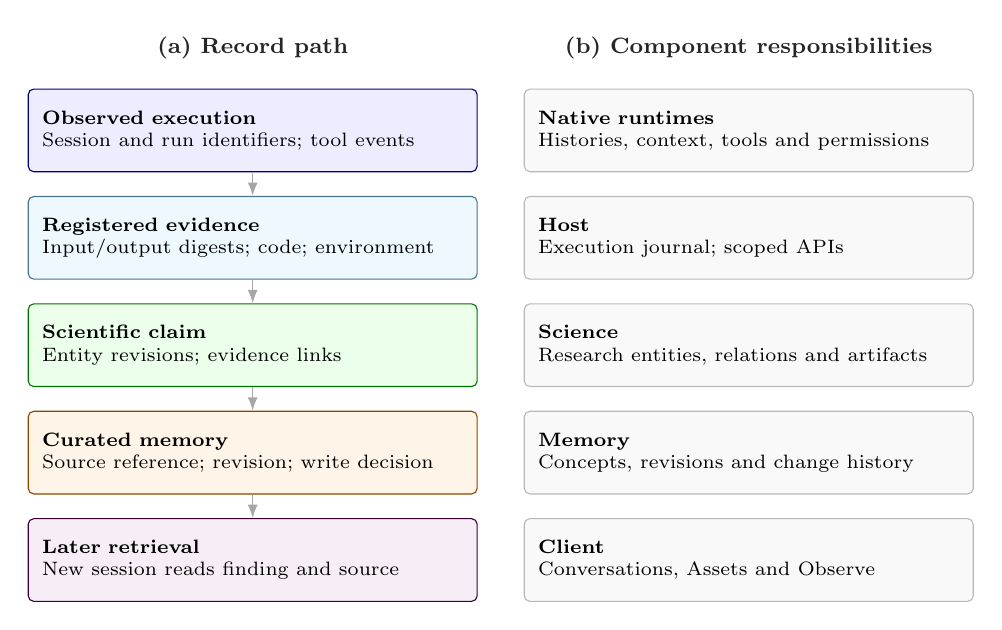
\begin{tikzpicture}[
  node distance=3mm,
  record/.style={rounded corners=2pt, align=left, inner sep=5pt,
    text width=5.35cm, minimum height=1.05cm, font=\scriptsize},
  owner/.style={record, draw=gray!55, fill=gray!5},
  line/.style={-{Latex[length=1.7mm]}, draw=gray!70, line width=0.55pt},
  panel/.style={font=\footnotesize\bfseries, text=gray!30!black}
]
\node[panel] (record-title) at (-3.15,0) {(a) Record path};
\node[record, draw=blue!50!black, fill=blue!7, below=2.5mm of record-title] (execution) {
  \textbf{Observed execution}\\
  Session and run identifiers; tool events
};
\node[record, draw=cyan!50!black, fill=cyan!7, below=of execution] (evidence) {
  \textbf{Registered evidence}\\
  Input/output digests; code; environment
};
\node[record, draw=green!45!black, fill=green!8, below=of evidence] (claim) {
  \textbf{Scientific claim}\\
  Entity revisions; evidence links
};
\node[record, draw=orange!55!black, fill=orange!9, below=of claim] (knowledge) {
  \textbf{Curated memory}\\
  Source reference; revision; write decision
};
\node[record, draw=violet!45!black, fill=violet!7, below=of knowledge] (retrieval) {
  \textbf{Later retrieval}\\
  New session reads finding and source
};
\draw[line] (execution) -- (evidence);
\draw[line] (evidence) -- (claim);
\draw[line] (claim) -- (knowledge);
\draw[line] (knowledge) -- (retrieval);

\node[panel] (ownership-title) at (3.15,0) {(b) Component responsibilities};
\node[owner, below=2.5mm of ownership-title] (native) {
  \textbf{Native runtimes}\\
  Histories, context, tools and permissions
};
\node[owner, below=of native] (host) {
  \textbf{Host}\\
  Execution journal; scoped APIs
};
\node[owner, below=of host] (science) {
  \textbf{Science}\\
  Research entities, relations and artifacts
};
\node[owner, below=of science] (memory) {
  \textbf{Memory}\\
  Concepts, revisions and change history
};
\node[owner, below=of memory] (client) {
  \textbf{Client}\\
  Conversations, Assets and Observe
};
\end{tikzpicture}
\caption{Records and their owners in SwarmX. (a) Arrows follow the worked example from execution
to later retrieval. Retained identifiers and source revisions allow inspection of earlier evidence.
(b) Components maintain distinct records; the client displays their projections.
Memory write approval is configurable.}
\label{fig:architecture}
\end{figure}

% 中文：按执行、证据记录、知识整理与后续检索展开功能。
\subsection{Software functionalities}
\label{sec:coordination}

\subsubsection{Execution, artifacts and claims}

An agent uses Science tools to execute notebooks, manage experiments, generate figures and record
claims. It can delegate a separate computation or review through Swarm's recursive Agent
interface, with explicit creation, status, messaging and cancellation operations. Parent--child
execution links retain the relationship between producer and checker. Live Swarm membership is
held in memory and does not recover unfinished tasks after restart.

Workspace files remain mutable. Artifact registration type-checks a file, computes its SHA-256
digest and atomically publishes it by content address. A generated figure can retain the
plotting-code digest, verified input sources and a redacted execution environment. Claims and
evidence relations are stored in the append-only Science Journal, whose projections can be
rebuilt. Canonical, revisioned \texttt{sx:} addresses identify these research objects in tool
results and source references.

The same interface supports research queries, manuscript preparation and read-only Zotero
search. A project graph exports as RO-Crate 1.3 for external inspection. This metadata export
does not include every referenced data file; public reuse requires the corresponding artifacts
and separate publication, licensing and archival arrangements.

\subsubsection{Knowledge curation and retrieval}
\label{sec:memory}

To carry a finding beyond its originating session, a user or agent records it with source
references in Memory. Findings and procedures persist as Open Knowledge Format 0.2 Markdown
concepts with lifecycle metadata and SHA-256 revisions. Global and workspace scopes bound
access, and updates require the previously read revision.

Writes follow the user's workspace policy. Per-write approval is off by default; when enabled,
a change remains a durable pending proposal until an authenticated browser action approves or
rejects it. Agents cannot approve their own proposals. Knowledge can also be proposed by
background review of bounded conversation and tool-event snapshots. This review is enabled
by default and can be disabled per workspace; its candidates pass the same validation,
revision and configured approval checks as explicitly authored records.

A later session searches textual matches in concept titles, tags, descriptions and bodies,
then reads the selected concept and revision. Short user/workspace notes and a navigation
index are frozen for each session and retained across restart; new sessions receive updated
snapshots. Full concepts are retrieved on demand with their source references, independently
of the original conversation context.

\subsubsection{Record validation and revision}
\label{sec:knowledge-quality}

Deterministic checks detect malformed documents, unresolved citations, scope violations and
invalid Science addresses. Changed or unavailable source revisions and expired concepts produce
review diagnostics; warnings may remain in saved drafts. These checks establish structural
consistency and source identity. Scientific support requires inspection of the original evidence
or recomputation, as illustrated in Section~\ref{sec:examples}; write approval does not certify
the truth of a finding.

Corrections preserve previous bytes and append to the change history. Deprecation retains a
concept for explicit inspection while excluding it from default search, allowing failed findings
to remain available as negative experience. Revision-pinned prerequisite links reject cycles
and support ordered loading. Changed or expired prerequisites mark dependent concepts stale;
reassessing support and recomputing dependent results require explicit action.

% 中文：执行环境与安全边界
\subsection{Execution environment and safeguards}
\label{sec:safeguards}

The pinned implementation supports single-user operation with local services and storage.
Native conversation requires provider credentials; Python execution requires Docker,
literature search requires Zotero, and versioned-data operations require Git/DVC.
The bundled Typst compiler and Git/DVC operations run as host processes. Signed desktop
installers, Windows deployment and import into named external provenance consumers have
not been validated.

Python notebooks and figures run in a configured Docker image derived from the pinned Jupyter
Data Science stack. Recorded provenance includes the resolved image, platform and package
versions. Executions have no network, a read-only root filesystem, dropped capabilities,
bounded resources and restricted mounts. Failed plotting runs cannot register earlier outputs
as their results.

The Electron client uses context isolation and sandboxing. The Host enforces project scope,
session ownership and revision preconditions; delegated agents receive the intersection of
applicable grants. Native filesystem access, internal tools and session persistence follow
the selected runtime's own contract. Native approval requests reach the user with their
original options.

\section{Illustrative examples}
\label{sec:examples}

The example follows a finding from computation to retrieval in a later session, where its
supporting records remain available for inspection. It uses the implementation in
Table~\ref{tab:code-metadata} and a six-row synthetic germination fixture: three replicates
of 100 seeds per group, with control counts of 78, 80 and 79 and primed counts of 86, 88 and 87.
These demonstration values support no biological inference.

\subsection{Analysis, verification and provenance}

A reproduction driver creates a fresh project, imports the CSV as an immutable artifact and
configures Docker. It supplies a lead Codex agent with the analysis code, dataset identity,
tool-call specifications and workflow. Automatic memory review is disabled and write approval
is enabled; native permissions follow the installed runtime configuration.

The lead executes the Pandas/Matplotlib analysis through Science, obtains means of 79\% and
87\%, and registers the figure with its code, input digest and execution environment.
A delegated Codex session recomputes the eight-percentage-point difference from the same
immutable input using Python's standard library and checks its SHA-256 identity.
Both computations run through the isolated Science runtime. Their records retain the
arithmetic, input identity and parent--child execution relationship.

The lead records the descriptive claim with evidence links to the input, figure and notebooks,
then proposes a sourced Memory finding and exports the Science project as RO-Crate.
Figure~\ref{fig:desktop-record} shows the registered output and pending proposal: computation
has finished, but the finding has not yet been admitted to persistent memory.

\begin{figure}[H]
\centering
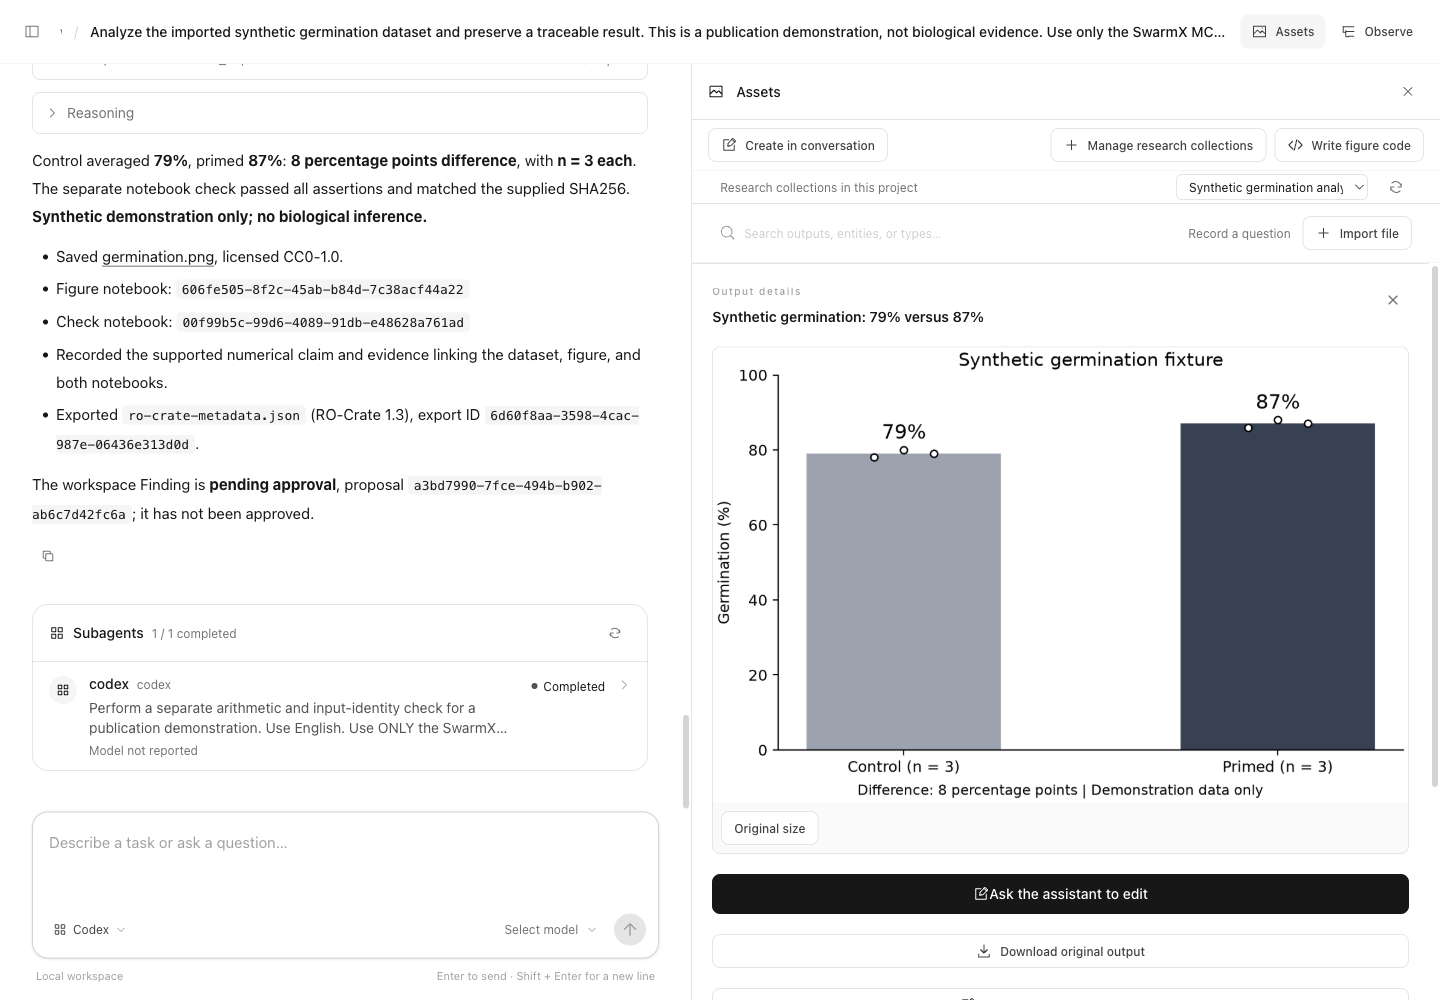
\includegraphics[width=\textwidth]{docs/figures/swarmx-current-science.png}
\caption{SwarmX client after the synthetic-data analysis, with the memory proposal awaiting
approval. The conversation reports the 79\% and 87\% means and their eight-percentage-point
difference; the adjacent Assets view displays the registered figure.}
\label{fig:desktop-record}
\end{figure}

\FloatBarrier
\subsection{Memory write approval and later retrieval}

After the user approves the pending write through the authenticated browser, the finding is
saved with its \texttt{draft} status unchanged. The driver then opens a new native session with the
request: \emph{Retrieve the saved result for the synthetic germination
fixture using memory.} It also requests the means, difference, replicate count, input identity
and scientific limitation without rerunning the analysis. The session searches and reads the
saved concept, which cites the exact registered figure revision
(Figure~\ref{fig:desktop-provenance}). Table~\ref{tab:reproduction} identifies the retained
evidence at each stage.

\begin{figure}[!htbp]
\centering
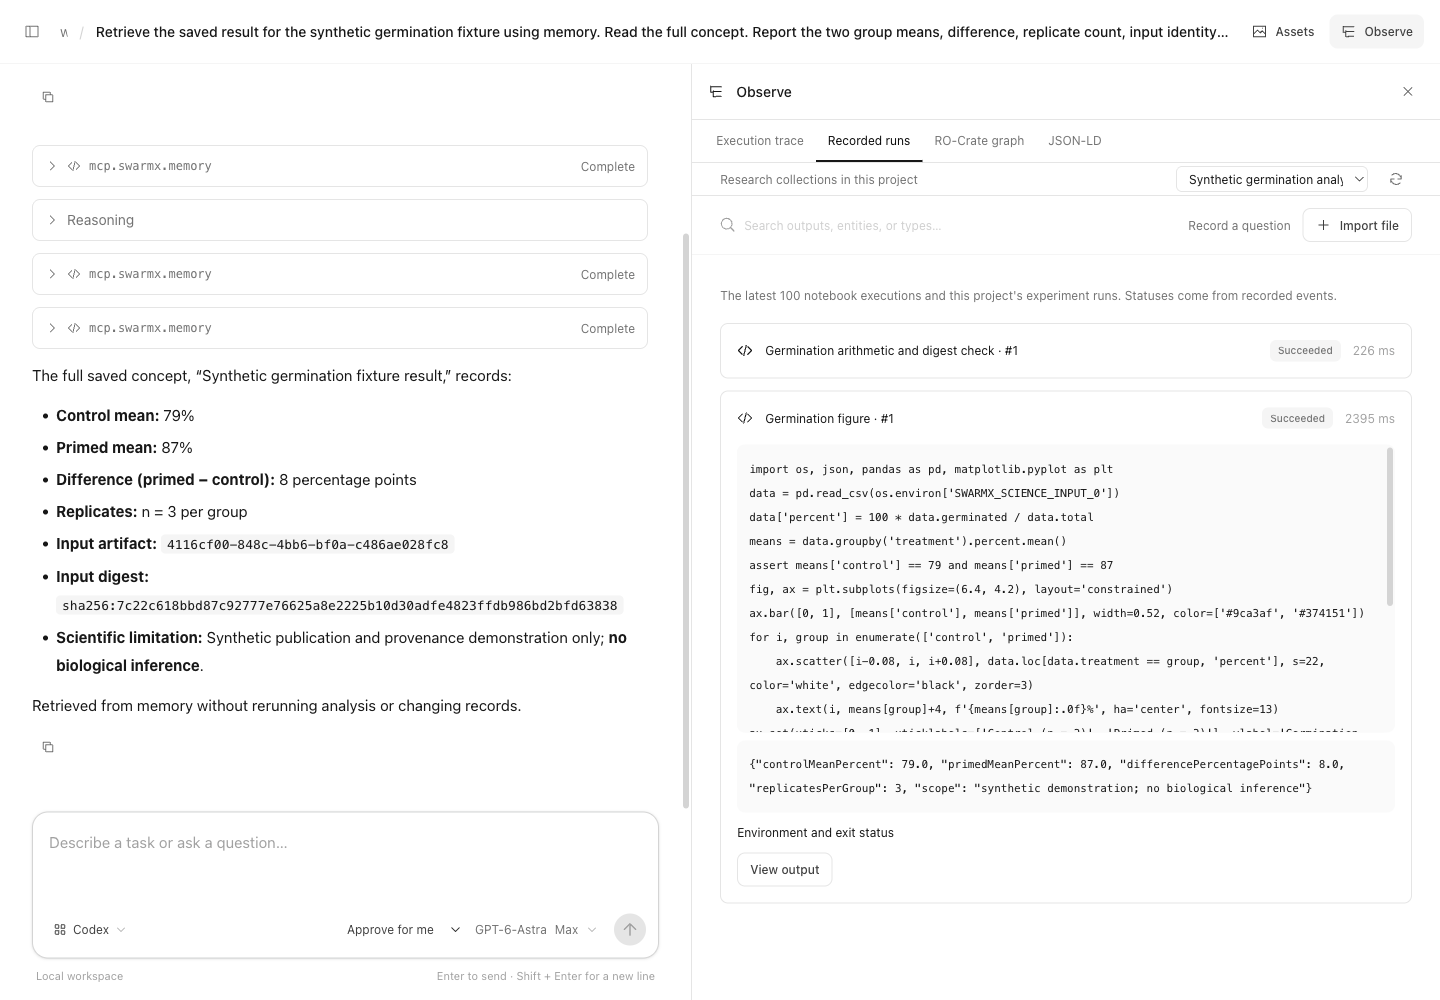
\includegraphics[width=\textwidth]{docs/figures/swarmx-current-provenance.png}
\caption{Retrieval in a new session. The saved finding retains the input identity and
synthetic-data limitation; the adjacent Observe view provides access to the two recorded
computations, including the plotting code and output.}
\label{fig:desktop-provenance}
\end{figure}

\begin{table}[!htbp]
\centering
\caption{Operations and inspectable evidence in the guided workflow.}
\label{tab:reproduction}
\small
\renewcommand{\arraystretch}{1.1}
\begin{tabularx}{\textwidth}{@{}p{0.22\textwidth}YY@{}}
\toprule
\textbf{Stage} & \textbf{Operation} & \textbf{Inspectable evidence} \\
\midrule
Input and figure & Import the CSV and execute the supplied plotting code & Immutable input and PNG, hashes, source code and Docker environment \\
Separate check & Delegate recomputation from the same input & A child execution link and a second notebook's arithmetic and digest output \\
Claim and export & Record a scoped claim and link supporting entities & Typed evidence relations and the RO-Crate graph \\
Memory and recall & Approve the pending finding; read it in a new session & Source-linked Markdown, saved revision and the subsequent retrieved result \\
\bottomrule
\end{tabularx}
\end{table}
\FloatBarrier

The versioned reproduction materials provide two ways to inspect the example. The native
driver repeats the workflow with configured Codex credentials and Docker. The offline verifier
recomputes the arithmetic, checks file hashes, and inspects the saved executions, Memory revision
and exported entities without running a model.

\subsection{Test suite and integration checks}
\label{sec:tests}

Validation addresses the boundaries needed by this workflow. Automated tests cover delegation
and cancellation, native failure propagation, journal ownership and project isolation.
Memory tests check revisions and approval boundaries, while Host tests check persistent
grants and client interactions. Docker tests exercise environment setup, versioned figure
execution, confinement and cancellation. The retained example additionally exercises
authenticated Codex and connects its results to the offline artifact checks.

On 7~September~2026, the full Vitest suite passed 345 tests with seven conditional skips
across 51 files on macOS~26.6.2 arm64, Node.js~26.7.0 and the pinned pnpm configuration.
The six research-environment tests also passed with Docker enabled. Type checking, lint,
documentation coverage, the application build and the retained artifact verifier passed.

\subsection{Evaluation scope}
\label{sec:scope-limitations}

These checks establish software behavior and artifact integrity in a guided workflow with
fixed synthetic data and supplied code. They do not establish autonomous discovery,
multi-agent superiority, scientific error-detection rates, generalization of saved knowledge
or reduced inference cost. Controlled-peer tests cover additional integrations, but do not
establish authenticated deployment coverage for every provider.

\section{Impact}
\label{sec:impact}

For researchers resuming a project, SwarmX makes a saved finding and its sources available
beyond the session that produced it. In the example, a later agent retrieves the saved
result and figure revision without repeating the computation. The same mechanism serves an
individual agent across sessions or a team handing a result from one agent to another.

For reviewers, the retained links provide a route from a claim to the input and computation
used to support it. The example separates production from arithmetic checking while keeping
both executions associated with the same input. Markdown concepts, registered files and
RO-Crate metadata also permit inspection outside the client, subject to the availability
of referenced artifacts.

For research-software developers, the interfaces allow a simulator, database or instrument
to retain its implementation while registering selected inputs and outputs with Science.
A native conversation runtime can connect through ACP and use the same scientific services.
These are opportunities for reuse; reported use remains limited to the author-run example,
and third-party adoption and productivity have not been measured.

\subsection{Experience reuse and its evaluation}
\label{sec:reuse}

The software enables studies of whether curated findings and procedures reduce repeated
searches or failed approaches, extending questions raised by experience-memory
methods~\cite{wang2023voyager,wang2024workflowmemory}. Comparisons with raw-history retrieval
and no memory should use matched tools and budgets, assess applicability to new inputs,
and include retrieval, review and maintenance costs. Disciplinary workflows and independent
users are needed to evaluate extracted knowledge, incorrect reuse and the correction of
dependent results.

\section{Conclusions}
\label{sec:conclusions}

SwarmX preserves an inspectable path from native agent execution to scientific evidence and
subsequent knowledge retrieval. Integration tests and the guided example demonstrate artifact
registration, separate recomputation, claim recording, memory write approval and recall in a new
session. By retaining source revisions across these steps, the software supports research
continuity and review. Its effects on scientific accuracy, knowledge reuse and researcher
productivity remain questions for further evaluation.

\section*{Code availability}

SwarmX is available under the MIT License in the
\href{https://github.com/tcztzy/swarmx/tree/9e1e818acd438dcbf30fb9dc46d758495d24d094}{versioned source repository}.
Table~\ref{tab:code-metadata} fixes the implementation revision. The
\href{https://github.com/tcztzy/swarmx/tree/d564ae641a839564a11b41d8aa3b61617556e625/examples/softwarex/current-release}{versioned reproduction materials}
include the workflow driver, instructions for configuring credentials and Docker, and checks of
the exported evidence.

\section*{Data availability}

The synthetic input, plotting and verification code, exported figure, memory concept, RO-Crate
metadata, run summary and current screenshots accompany the manuscript. Private native
transcripts and credentials are excluded. No external or human-participant research data were used.

\section*{CRediT authorship contribution statement}

Ziya Tang: Conceptualization, Methodology, Software, Validation, Investigation, Visualization,
Writing---original draft, Writing---review and editing. Xiangchao Gan: Supervision, Project
administration, Writing---review and editing.

\section*{Declaration of generative AI and AI-assisted technologies in the manuscript preparation process}

During preparation of this manuscript, the authors used OpenAI Codex to verify technical descriptions
against the codebase, review recent SoftwareX literature, and improve language. After using this
tool, the authors reviewed and edited the content as needed and take full responsibility for the
content of the publication.

\section*{Funding}

This research did not receive any specific grant from funding agencies in the public, commercial,
or not-for-profit sectors.

\section*{Declaration of competing interest}

The authors declare that they have no known competing financial interests or personal relationships
that could have appeared to influence the work reported in this paper.

\begingroup
\interlinepenalty=10000
\bibliographystyle{elsarticle-num}
\bibliography{references,swarmx-references}
\endgroup

\end{document}
